% Options for packages loaded elsewhere
\PassOptionsToPackage{unicode}{hyperref}
\PassOptionsToPackage{hyphens}{url}
%
\documentclass[
  11pt,
  a4paper,
]{article}
\usepackage{amsmath,amssymb}
\usepackage{lmodern}
\usepackage{iftex}
\ifPDFTeX
  \usepackage[T1]{fontenc}
  \usepackage[utf8]{inputenc}
  \usepackage{textcomp} % provide euro and other symbols
\else % if luatex or xetex
  \ifXeTeX
    \usepackage{zxjatype} 
    \usepackage[ipaex]{zxjafont}
    \setromanfont{Times New Roman}
  \fi
  \usepackage{unicode-math}
  \defaultfontfeatures{Scale=MatchLowercase}
  \defaultfontfeatures[\rmfamily]{Ligatures=TeX,Scale=1}
\fi
% Use upquote if available, for straight quotes in verbatim environments
\IfFileExists{upquote.sty}{\usepackage{upquote}}{}
\IfFileExists{microtype.sty}{% use microtype if available
  \usepackage[]{microtype}
  \UseMicrotypeSet[protrusion]{basicmath} % disable protrusion for tt fonts
}{}
\usepackage{xcolor}
\IfFileExists{xurl.sty}{\usepackage{xurl}}{} % add URL line breaks if available
\IfFileExists{bookmark.sty}{\usepackage{bookmark}}{\usepackage{hyperref}}
\hypersetup{
  pdftitle={Estimating Effect of Tax Incentives on Donations Considering Self-Selection of Tax Incentives in South Korea},
  hidelinks,
  pdfcreator={LaTeX via pandoc}}
\urlstyle{same} % disable monospaced font for URLs
\usepackage[left=3cm,right=3cm,top=3cm,bottom=3cm]{geometry}

\usepackage{setspace}
\renewcommand{\baselinestretch}{1.5}
\usepackage{float}

\usepackage{longtable,booktabs,array}
\usepackage{threeparttable, threeparttablex, multirow}
\usepackage{calc} % for calculating minipage widths
% Correct order of tables after \paragraph or \subparagraph
\usepackage{etoolbox}
\makeatletter
\patchcmd\longtable{\par}{\if@noskipsec\mbox{}\fi\par}{}{}
\makeatother
% Allow footnotes in longtable head/foot
\IfFileExists{footnotehyper.sty}{\usepackage{footnotehyper}}{\usepackage{footnote}}
\makesavenoteenv{longtable}
\usepackage{graphicx}
\makeatletter
\def\maxwidth{\ifdim\Gin@nat@width>\linewidth\linewidth\else\Gin@nat@width\fi}
\def\maxheight{\ifdim\Gin@nat@height>\textheight\textheight\else\Gin@nat@height\fi}
\makeatother
% Scale images if necessary, so that they will not overflow the page
% margins by default, and it is still possible to overwrite the defaults
% using explicit options in \includegraphics[width, height, ...]{}
\setkeys{Gin}{width=\maxwidth,height=\maxheight,keepaspectratio}
% Set default figure placement to htbp
\makeatletter
\def\fps@figure{htbp}
\makeatother
\setlength{\emergencystretch}{3em} % prevent overfull lines
\providecommand{\tightlist}{%
  \setlength{\itemsep}{0pt}\setlength{\parskip}{0pt}}
\setcounter{secnumdepth}{5}
\newlength{\cslhangindent}
\setlength{\cslhangindent}{1.5em}
\newlength{\csllabelwidth}
\setlength{\csllabelwidth}{3em}
\newlength{\cslentryspacingunit} % times entry-spacing
\setlength{\cslentryspacingunit}{\parskip}
\newenvironment{CSLReferences}[2] % #1 hanging-ident, #2 entry spacing
 {% don't indent paragraphs
  \setlength{\parindent}{0pt}
  % turn on hanging indent if param 1 is 1
  \ifodd #1
  \let\oldpar\par
  \def\par{\hangindent=\cslhangindent\oldpar}
  \fi
  % set entry spacing
  \setlength{\parskip}{#2\cslentryspacingunit}
 }%
 {}
\usepackage{calc}
\newcommand{\CSLBlock}[1]{#1\hfill\break}
\newcommand{\CSLLeftMargin}[1]{\parbox[t]{\csllabelwidth}{#1}}
\newcommand{\CSLRightInline}[1]{\parbox[t]{\linewidth - \csllabelwidth}{#1}\break}
\newcommand{\CSLIndent}[1]{\hspace{\cslhangindent}#1}


\usepackage{booktabs}
\usepackage{longtable}
\usepackage{array}
\usepackage{multirow}
\usepackage{wrapfig}
\usepackage{float}
\usepackage{colortbl}
\usepackage{pdflscape}
\usepackage{tabu}
\usepackage{threeparttable}
\usepackage{threeparttablex}
\usepackage[normalem]{ulem}
\usepackage{makecell}
\usepackage{xcolor}
\usepackage{siunitx}
\newcolumntype{d}{S[input-symbols = ()]}
\ifLuaTeX
  \usepackage{selnolig}  % disable illegal ligatures
\fi

\makeatletter
\def\@fnsymbol#1{\ensuremath{\ifcase#1\or \dagger\or \ddagger\or
   \mathsection\or \mathparagraph\or \|\or **\or \dagger\dagger
   \or \ddagger\ddagger \else\@ctrerr\fi}}
    \makeatother
\title{Estimating Effect of Tax Incentives on Donations Considering Self-Selection of Tax Incentives in South Korea  }
\author{
    Hiroki Kato
  \thanks{Graduate School of Economics, Osaka University, Japan. E-mail: h-kato@econ.osaka-u.ac.jp  }
  \and
    Tsuyoshi Goto
  \thanks{Graduate School of Social Sciences, Chiba University, Japan. E-mail: t.goto@chiba-u.jp  }
  \and
    Youngrok Kim
  \thanks{Graduate School of Economics, Kobe University, Japan.  }
  \and
  }

\date{2022/04/19}


\begin{document}
\begin{spacing}{1}
  \maketitle
\end{spacing}

\hypertarget{intro}{%
\section{Introduction}\label{intro}}

In many countries, governments set a tax relief for charitable giving.
This is because, if subsidizing charitable giving induces a large increase in donations,
it is desirable for public good provision.
As Saez (2004) shows,
it is known that
the elasticity of charitable donations
respect to the giving price relative to the private consumption (giving price, hereafter) is
a key parameter to evaluate the welfare implication.
To receive the tax relief, tax payers have to declare their charitable giving to tax agency.
Then, giving price will be reduced from one to one minus the marginal income tax rate
(if the tax relief is applied through deduction) or one minus the credit rate (if tax credit).

Starting with Feldstein (1975),
there are a large empirical literature examining the giving price elasticity.
Papers in this literature regress the log-valued giving price on
the log-valued amount of charitable giving
to derive the giving price elasticity
using tax filing data
(e.g.~Randolph, 1995; Auten et al., 2002; Fack and Landais, 2010; Bakija and Heim, 2011; Almunia et al., 2020)
or panel survey data (e.g.~Rehavi and Shack, 2013; Yoruk, 2013; Zampelli and Yen, 2016; Backus and Grant, 2019).
Although many of these papers consider the endogeneity issue
such as the endogenous change of the marginal tax rate by the amount of giving,
they pay less attention to the problems caused by the fact that
tax payers have to declare their charitable giving to receive tax relief on charitable giving.
Therefore, if the estimation ignores the declaration of charitable giving,
the self selection bias happens to the estimation
in the sense that the charitable giving is declared by
only those who can expect benefits from the charitable giving or
those who have the giving preference.
To our knowledge,
no paper in the literature considers the self selection
about the declaration of charitable giving.\footnote{Although Almunia et al.~(2020) consider
  the self selection process about the declaration of charitable giving as an exception,
  their reduced-form estimation about the giving price elasticity
  does not consider the self selection.
  They use the giving price elasticities estimated by the reduced-form analysis to
  structurally estimate a fixed compliance cost for declaration,
  where they consider the self selection process.}

Considering that the application of tax relieves is based on self declaration,
the self selection problem is caused by
the existence of compliance costs to apply measures of tax relives
because everyone will apply the measures if there is no compliance cost.
In other words, if there are the compliance costs,
tax payers apply the measures of tax relives only if
their benefits from the measures exceed the compliance costs.
In the literature of tax compliance,
recent papers insist this point and suggest that
the measures of tax relives may not work as
the policy makers expected
since the application of the measures entails compliance costs.
They also suggest compliance costs,
which include record-keeping cost and a fee for accountants,
are considerably high.\footnote{For the individual income tax,
  Benzarti (2020) estimates that the cost of the income tax filing is
  0.6-0.8 percent of adjusted gross income in the U.S..
  For the corporate income tax,
  Zwick(2021) finds that only 37 percent of eligible firms claim
  their refund in their corporate tax returns because of the complexity of tax code.}
In the context of charitable giving,
some papers also suggest the existence of compliance costs to declare charitable giving.
Fack and Landais (2016) study a 1983 reform in France,
which introduced the requirement to submit the certification,
and find the significant reduction of
the declaration of charitable giving after 1983.\footnote{They also show that
  the estimated price elasticity changed before and after the reform.
  This is because the declaration of charitable giving dramatically
  reduced after the reform and they use tax filer data.}
Gillitzer and Skov (2018) examine a 2008 reform in Demmark,
which allowed charities to pre-populate the tax record with the donation record
in order to reduce declaration costs,
and find a large increase of charitable giving declaration after the reform.
Almunia et al.~(2020)
estimate the amount of a fixed compliance cost in the U.K.,
which is estimated as £47.

Although several papers suggest
the existence of compliance costs in the tax compliance literature,
no paper in the literature of giving price elasticity consider the self selection problem.
Therefore, this paper tries to fill this gap and
estimates the giving price elasticity
using the South Korean (Korea, hereafter) survey panel data
called the National Survey of Tax and Benefit (NaSTaB).
The usage of this data brings us to three advantages on the estimation.
Firstly, for the issue of self selection,
we utilize an instrument variable (IV)
which represents the compliance cost for charitable giving declaration.
In the Korean tax system, to receive tax relief,
wage earners can declare tax relief in their company at any time
while self-employed workers have to declare tax relief in the tax agency
at a time of tax return.
Wage earners do not need understand the tax system nor
keep the certification of donation until the tax return season
since their company deals with tax business instead of them
and they can submit the certification at any time.
Self-employed workers, on the other hand, have to understand the tax system
and keep the certification.
Therefore, there is a difference of the compliance cost
between wage earners and self-employed workers.
Whether tax payers are wage earners and self-employed workers is
determined irrespective to their expected benefit from charitable giving or giving preference,
while the different compliance costs between them will make
a difference about the behavior of the declaration.
Instrumented by the wage earner dummy,
the declaration of charitable giving will be less affected
by the benefit from the declaration.
One of the advantages of our IV is that
the compliance costs are not considered to have a direct impact on a giving behavior
although they have a effect on it through the declaration of charitable giving.
Since the difference in compliance cost has no effect on the giving behavior
if there is no declaration system of charitable giving,
tax payers' giving behavior innately have no relation to the compliance cost.
As for another advantage of our IV,
the causality from the compliance cost to the charitable giving declaration
seems credible and their relation is monotone since recent papers
such as Fack and Landais (2016) and Gillitzer and Skov (2018) imply that the existence of compliance costs significantly reduce the declaration of charitable giving.\footnote{In addition,
  another advantage of our setting is that
  we can capture the heterogeneity of compliance costs,
  while all taxpayers experience the change of compliance costs
  in the setting of Fack and Landais (2016) and Gillitzer and Skov (2018).
  (これdiscussionに持ってっても良いかも)}

Secondly, we address the issue of sample selection bias using the panel survey data.
Considering that the giving price is dependent on the declaration of charitable giving
we have to distinguish declared and undeclared charitable giving.
However, tax return data,
which is used in many papers in the literature of giving price elasticity,
do not record undeclared charitable giving and giving by tax withholders.
In addition,
since those who itemize their giving tends to be wealthier than the average taxpayer,
the estimates based on tax filer data will represent the behaviors of high-income earners.
Panel survey data contains information about charitable giving
irrespective of tax filing or giving declaration.
The estimation using panel survey data should be free from
the sample selection bias (Rehavi and Shack, 2013; Backus and Grant, 2019).
Since NaStaB data is constructed by reflecting the Korean society,
we could consider the sample of low-income households,
which are sometimes omitted from the tax filer data.
This is particularly important for the estimation of the price elasticity
in terms of the extensive margin
since the propensity of donation by low-income earners
tend to be less than high-income earners.

Thirdly, to derive the elasticity,
this paper exploits the South Korean tax reform in 2014
as a main identification strategy.
In the 2014 reform,
tax credit was introduced as a way for the tax relief on charitable giving,
though income deduction had been used before.
The 2014 tax reform started to allow 15\% of the total amount of charitable giving
as a tax credit for all declaring taxpayers,
which means that the giving price for 1 KRW donation is 0.85 KRW.\footnote{1 KRW is approximately 0.001 USD. In other words, 1 USD is about 1,000 KRW.}
Since the giving price was determined according to the marginal tax rate of
progressive income tax before 2014,
this tax reform reduced the giving price for low income taxpayers
while it increased the price for high income tax payers.
Since the variation of giving price can be considered to be exogenous for taxpayers,
we exploit this reform and conduct the difference-in-difference (DID) analysis
for identification.\footnote{To our knowledge,
  only Hong(2020) considers the policy change(s) in Korea using panel data
  and derives the estimated giving price elasticity as -1.2.
  However, he does not use DID nor consider the self selection bias.}

Using the IV representing the compliance cost,
the estimated giving price elasticities are in the range between XXX and XXX
in terms of intensive-margins.
If the IV is not used,
we find that the estimated intensive-margins giving price elasticity is XXX,
which is similar value to the estimates in the existing literature.
Considering that those who can expect benefits from the charitable giving and
who have the giving preference are less affected by the change of the giving price,
OLS estimates may overestimate their effects.
As for the extensive-margins giving price elasticity,
the estimates with the IV are in the range between XXX and XXX,
while the estimate without the IV is XXX.
The extensive margins elasticity shows
whether tax payers donate or not depending on the giving price.
Since those who stop donating will not declare their donation and
their giving price will increase to one,
if the endogeneity of declaration is not considered,
the estimates will be elastic and it will be interpreted
as if the donation is stopped by the increase of the giving price.
The usage of the IV prevents a possibility of such a reverse causality.

In addition,
the estimation of the intensive-margins and extensive-margins giving price elasticity considers
well-known challenges for the estimations in this literature
such as the endogenous change of the marginal tax rate by the amount of giving,
simultaneous determination of income and donation and the announcement effect of policy change.
We examine all of these issues in the robustness check and
find that the intensive-margin tax-price elasticities are in the range of -2 and -1.5
and the extensive-margin tax-price elasticities are in the range of -5 and -1.7
in the almost all cases of the estimations.

This paper consists of six sections.
Section 2 and 3 respectively explain the institutional background and data.
Section 4 explains the estimation method.
Section 5 deals with the analysis of price elasticity.
Section 6 concludes.

\hypertarget{background}{%
\subsection{Institutional background and Sources of Endogeneity}\label{background}}

In this section,
we describe the income tax relief for charitable giving in Korea
and the endogeneity issues arising from the declaration of giving.

\hypertarget{system-of-tax-relief-on-charitable-giving}{%
\subsection{System of tax relief on charitable giving}\label{system-of-tax-relief-on-charitable-giving}}

To explain how income tax relief on charitable giving is applied and
how the giving price is determined,
we introduce a abstract framework in this subsection.
Thus, let us consider that a household with pre-tax income \(y_i\)
has a choice between private consumption \(x_i\) and charitable giving \(g_i\).
Their budget constraint can be shown as
\begin{align}
x_i + g_i = y_i − R_iK_i - R_iT(y_i, g_i) - (1-R_i)T(y_i). \label{eq:budget}
\end{align}
\(T\) is tax amount which depends on the pre-tax income and charitable giving.
Since the marginal income tax rate is progressive in Korea,
we assume \(T(\cdot)\) satisfy \(T_y(\cdot)>0\) and \(T_{yy}(\cdot)>0\) hereafter,
where the subscript means the partial differentiation.
\(R_i\) is the dummy which takes 1 if \(i\) declares the tax relief and 0 otherwise.
\(K_i\) is a fixed compliance cost for the declaration of charitable giving.
While \(K_i\) includes non-monetary cost such as record-keeping cost and
monetary cost such as a fee for accounts,
it is converted to pecuniary terms for simplicity.
In the literature about the giving price elasticity,
since most of papers implicitly assume \(R_i=1\) and \(K_i=0\).

Tax payers can reduce their income tax payment by declaring their giving.
However, the declaration entails the fixed compliance cost \(K_i\).
Therefore, whether tax payers declare their giving or not is determined according to
\begin{align}
  R_i = \begin{cases}
      1 \text{ if }T(y_i, g_i) + K_i<T(y_i)\\
      0 \text{ if }T(y_i, g_i) + K_i\ge T(y_i). \label{eq:R}
  \end{cases}
\end{align}
When tax payers do not declare their giving, the amount of income tax will be \(T(y_i)\).
When tax payers declare their giving, the amount of tax is
\begin{align}
  T(y_i, g_i) =
  \begin{cases} 
      T(y_i-g_i)&\text{ if tax relief is applied by income deduction.}\\
      T(y_i)-mg_i &\text{ if tax relief is applied by tax credit.} \label{eq:relief}
  \end{cases}
\end{align}

To derive the giving price,
let us differentiate the budget constraint \eqref{eq:budget} by \(x_i\) and \(g_i\).
Then, it derives that the giving price
(relative to the private consumption) is
\(\frac{dx_i}{dg_i}=1+R_iT_g(y_i,g_i)\),
which we denote \(p\).
Therefore, according to \eqref{eq:relief},
the giving price \(p\) is
\begin{align}
    p=
    \begin{cases} 
        1-R_iT'(y_i-g_i)&\text{ if tax relief is applied by income deduction.}\\
        1-R_im&\text{ if tax relief is applied by tax credit.}\label{giving price}
    \end{cases}
\end{align}
Hereafter,
let us \(q\) to show the amount of tax relief for each declared giving
(i.e.~\(p=1-R_iq\) and \(q=-T_g(y_i, g_i)\)).
The government can change \(q\) by the tax reform as the next subsection explains.

\begin{table}

\caption{\label{tab:mtr}Marginal Income Tax Rate}
\centering
\fontsize{9}{11}\selectfont
\begin{threeparttable}
\begin{tabular}[t]{lccccccc}
\toprule
Income/Year & 2008 & 2009 & 2010 \textasciitilde{} 2011 & 2012 \textasciitilde{} 2013 & 2014 \textasciitilde{} 2016 & 2017 & 2018\\
\midrule
(A) \textasciitilde{} 1200 & 8\% & 6\% & 6\% & 6\% & 6\% & 6\% & 6\%\\
\cmidrule{1-8}
(B) 1200 \textasciitilde{} 4600 & 17\% & 16\% & 15\% & 15\% & 15\% & 15\% & 15\%\\
\cmidrule{1-8}
(C) 4600 \textasciitilde{} 8800 & 26\% & 25\% & 24\% & 24\% & 24\% & 24\% & 24\%\\
\cmidrule{1-8}
(D) 8800 \textasciitilde{} 15000 &  &  &  &  & 35\% &  & 35\%\\
\cmidrule{1-1}
\cmidrule{6-6}
\cmidrule{8-8}
(E) 15000 \textasciitilde{} 30000 &  &  &  & \multirow{-2}{*}{\centering\arraybackslash 35\%} &  & \multirow{-2}{*}{\centering\arraybackslash 35\%} & 38\%\\
\cmidrule{1-1}
\cmidrule{5-5}
\cmidrule{7-8}
(F) 30000 \textasciitilde{} 50000 &  &  &  &  &  & 38\% & 40\%\\
\cmidrule{1-1}
\cmidrule{7-8}
(G) 50000 \textasciitilde{} & \multirow{-4}{*}{\centering\arraybackslash 35\%} & \multirow{-4}{*}{\centering\arraybackslash 35\%} & \multirow{-4}{*}{\centering\arraybackslash 35\%} & \multirow{-2}{*}{\centering\arraybackslash 38\%} & \multirow{-3}{*}{\centering\arraybackslash 38\%} & 40\% & 42\%\\
\bottomrule
\end{tabular}
\begin{tablenotes}
\item Notes: Marginal income tax rates applied from 2008 to 2018 are summarized.
  The income level is shown in terms of 10,000 KRW,
  which is approximately 10 United States dollars (USD)
  at an exchange rate of 1,000 KRW to one USD.
\end{tablenotes}
\end{threeparttable}
\end{table}

\hypertarget{taxreform}{%
\subsection{Korean tax system and tax reform in 2014}\label{taxreform}}

Korean tax system offers a tax relief for charitable giving in income tax.
To mitigate the administrative cost,
the Korean National Tax Service introduce different taxation methods
and different ways of giving declaration for wage earners and self-employed workers.
Wage earners pay income tax by tax withholding and
can declare their giving via their company at anytime
since, instead of them, their company is supposed to
close the comprehensive income tax return including giving declaration
through year-end settlement.
Self-employed workers have to calculate the amount of income
earned during a year and pay income tax through tax return by May of the following year.
To receive tax relief on charitable giving,
they have to submit the certificate of donations when they submit tax return.
Therefore, there is a difference of compliance cost of tax relief
since self-employed workers have to understand tax system to precisely populate tax return
and retain the certificate until they submit tax return
although wage earners need not to understand tax system and
can submit the certificate at any time.

Before 2014, tax relief on charitable giving is conducted by income deduction in Korea.
Since the marginal income tax rate was progressively determined as Table \ref{tab:mtr},
tax payer facing the higher marginal income tax rate
can enjoy the lower giving price for each 1 KRW of donation,
i.e.~the giving price was regressive before 2014.
In 2014, aiming at the relaxation of regressivity of giving price,
the Korean government reformed tax system,
where the tax credit was introduced instead of income deduction.
Since then, 15\% of the total amount of charitable giving has been allowed as a tax credit,
which means that the giving price from 2014 is 0.85 KRW
for each 1 KRW of donation irrelevant to the income level.
Therefore, compared to tax credit system,
the high income household,
whose (average) income tax rate is more than 15\%,
get benefit from charitable giving under the income deduction system.
However, middle or low income households would enjoy tax relief in tax credit system
more than income deduction system.
We exploit the variation of giving price brought from the policy change
as a main identification source to estimate the giving price elasticity.

\hypertarget{nastab}{%
\section{Data: National Survey of Tax and Benefit (NaSTaB)}\label{nastab}}

本研究は2008年からKorea Institute of Taxation and Financeが実施した
National Survey of Tax and Benefit (NaSTaB)を用いる。
これは家計の税負担や公的扶助などに関する年次パネルデータである。
この調査は全国から5,634世帯を対象とし、
5,634人の世帯主と15歳以上で経済活動をしている世帯員が調査に回答する。
この調査は前年の所得や寄付額に関する情報を含んでおり、
それらに加えて、教育年数などの個人属性や税制に対する個人の意識に関する情報を含んでいる。

\begin{table}
\centering
\fontsize{9}{11}\selectfont
\begin{tabular}[t]{lccc}
\toprule
  & N & Mean & Std.Dev.\\
\midrule
\addlinespace[0.3em]
\multicolumn{4}{l}{\textbf{Income and giving price}}\\
\hspace{1em}Annual taxable labor income (unit: 10,000KRW) & 36189 & \num{1747.26} & \num{2696.77}\\
\hspace{1em}First giving relative price & 36198 & \num{0.86} & \num{0.04}\\
\addlinespace[0.3em]
\multicolumn{4}{l}{\textbf{Charitable giving}}\\
\hspace{1em}Annual chariatable giving (unit: 10,000KRW) & 36199 & \num{35.64} & \num{153.20}\\
\hspace{1em}Dummary of donation > 0 & 36199 & \num{0.24} & \num{0.42}\\
\hspace{1em}Dummy of declaration of a tax relief & 36199 & \num{0.10} & \num{0.30}\\
\addlinespace[0.3em]
\multicolumn{4}{l}{\textbf{Individual Characteristics}}\\
\hspace{1em}Age & 36199 & \num{53.45} & \num{16.22}\\
\hspace{1em}Female dummy & 36199 & \num{0.43} & \num{0.50}\\
\hspace{1em}University graduate & 36198 & \num{0.42} & \num{0.49}\\
\hspace{1em}High school graduate dummy & 36198 & \num{0.31} & \num{0.46}\\
\hspace{1em}Junior high school graduate dummy & 36198 & \num{0.27} & \num{0.44}\\
\hspace{1em}Wage earner dummy & 27394 & \num{0.56} & \num{0.50}\\
\bottomrule
\end{tabular}
\end{table}

我々の研究では(1)2013年から2018年かつ、(2)23歳以下の回答者を除いたデータを使用する。
データの期間を制限した理由は、2014年の制度改革に注目するためである。
所得控除制度が適用されている期間(2014年の制度改革前)では、所得税率の改正が寄付行動に影響を与える。
この制度が適用されている期間において、所得税率の改正は2011年が最後である。
したがって、2011年以前の寄付行動を用いると、2014年の制度改革以外の影響を含んでしまう。
その可能性を取り除くために、我々は2013年から2018年のデータ(2012年から2017年の寄付行動)を用いる。
また、23歳以下の回答者を除いた理由は、所得や資産を十分に持っていない可能性が高いからである。
表\ref{tab:SummaryCovariate}に記述統計を示した。

\begin{figure}[t]

{\centering 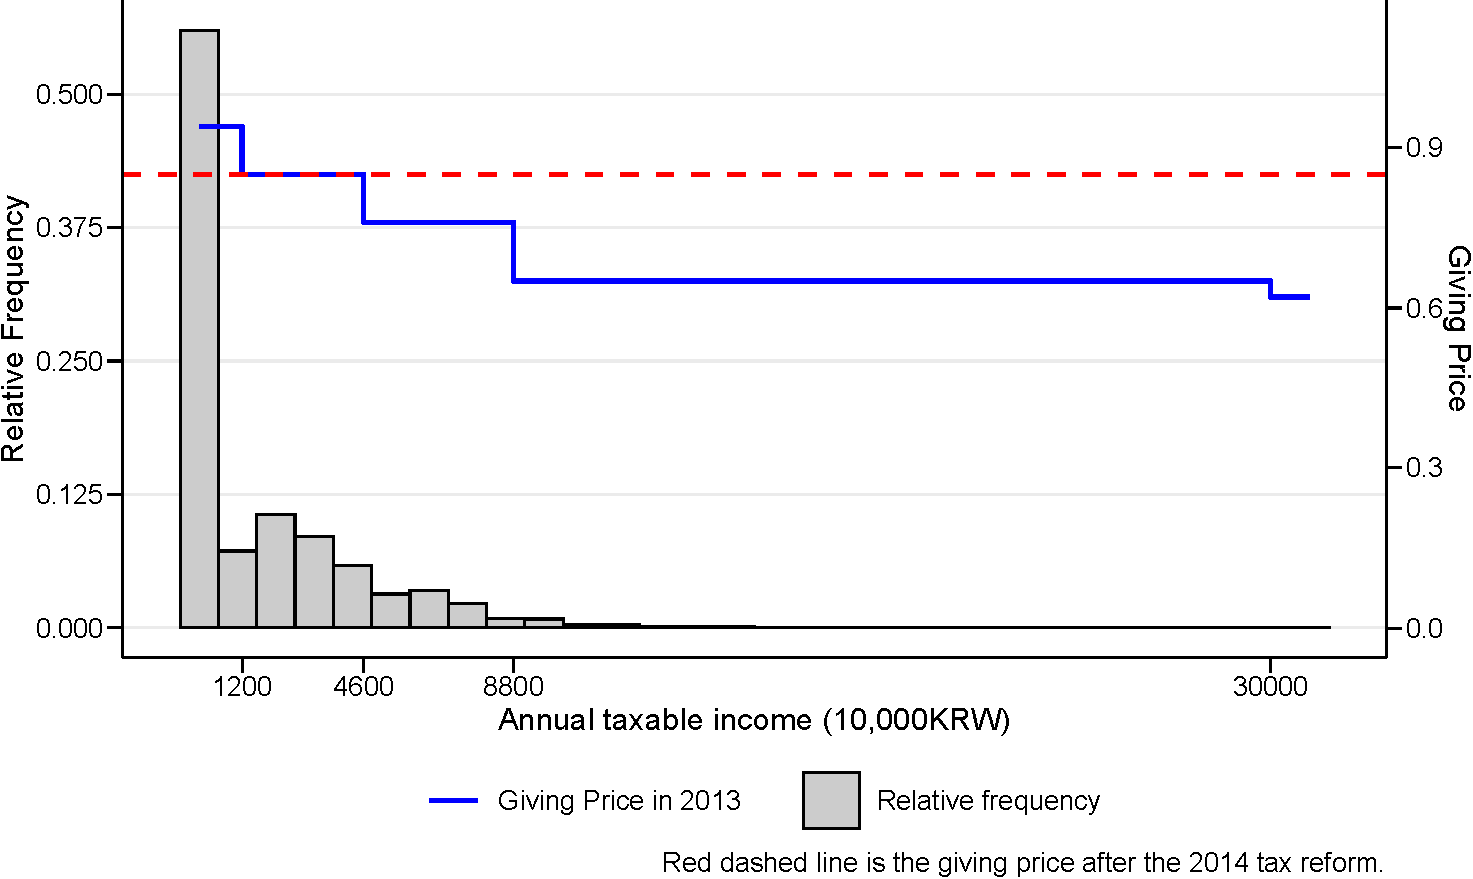
\includegraphics{C:/Users/vge00/Desktop/NaSTaB/docs/paper/body_files/figure-latex/SummaryPrice-1} 

}

\caption{Income Distribution in 2013 and Relative Giving Price. Notes: The left and right axis measure the relative frequency of respondents (grey bars) and the relative giving price (solid step line and dashed line), respectively. A solid step line and a dashed horizontal line represents the giving price in 2013 and 2014, respectively.}\label{fig:SummaryPrice}
\end{figure}

NaSTabは前年の労働所得を調査している。
表\ref{tab:SummaryCovariate}は、
我々が用いるサンプルの労働所得の平均額は17.54 million KRWであることを示しており、
Korean National Tax Serviceが発行しているNational Tax Statistical Yearbook 2012-2018
の平均所得32.77 million KRWより低い。
これはNaSTaBが主婦などの労働所得がない人を含んでいるからである。
したがって、所得分布は右歪曲な分布になる(図\ref{fig:SummaryPrice})。
我々は労働所得に基づいて限界税率を計算し、所得控除における寄付価格を計算した。
図\ref{fig:SummaryPrice}の黒の実線は2012年から2013年の寄付の相対価格を示している。

また、図\ref{fig:SummaryPrice}は価格弾力性を識別するための価格変動も示している。
先に述べたように、黒の実線は所得控除が適用されている期間(2012年から2013年)の寄付の相対価格を示している。
対して、黒の破線は税額控除が適用されている期間(2014年以降)の寄付の相対価格を示している。
2014年の税制改革による税インセンティブの変化に基づいて、我々は三つの所得グループを作ることができる:
(1) 120 million KRWより低い;
(2) 120 million KRWから460 million KRWの間;
(3) 460 million KRWより高い。
第一のグループに属する人の税インセンティブは税制改革によって拡大した(寄付価格が減少した)。
第二のグループに属する人の税インセンティブは税制改革によって変化しなかった。
第三のグループに属する人の税インセンティブは税制改革によって縮小した(寄付価格が増加した)。
このグループによる差分の差分法が我々の第一の識別戦略となる\footnote{2011年以前の寄付行動は所得税率の改正による影響をうけるので、税制改革前の平行トレンドを検証することはできない。}。

\begin{figure}[t]

{\centering 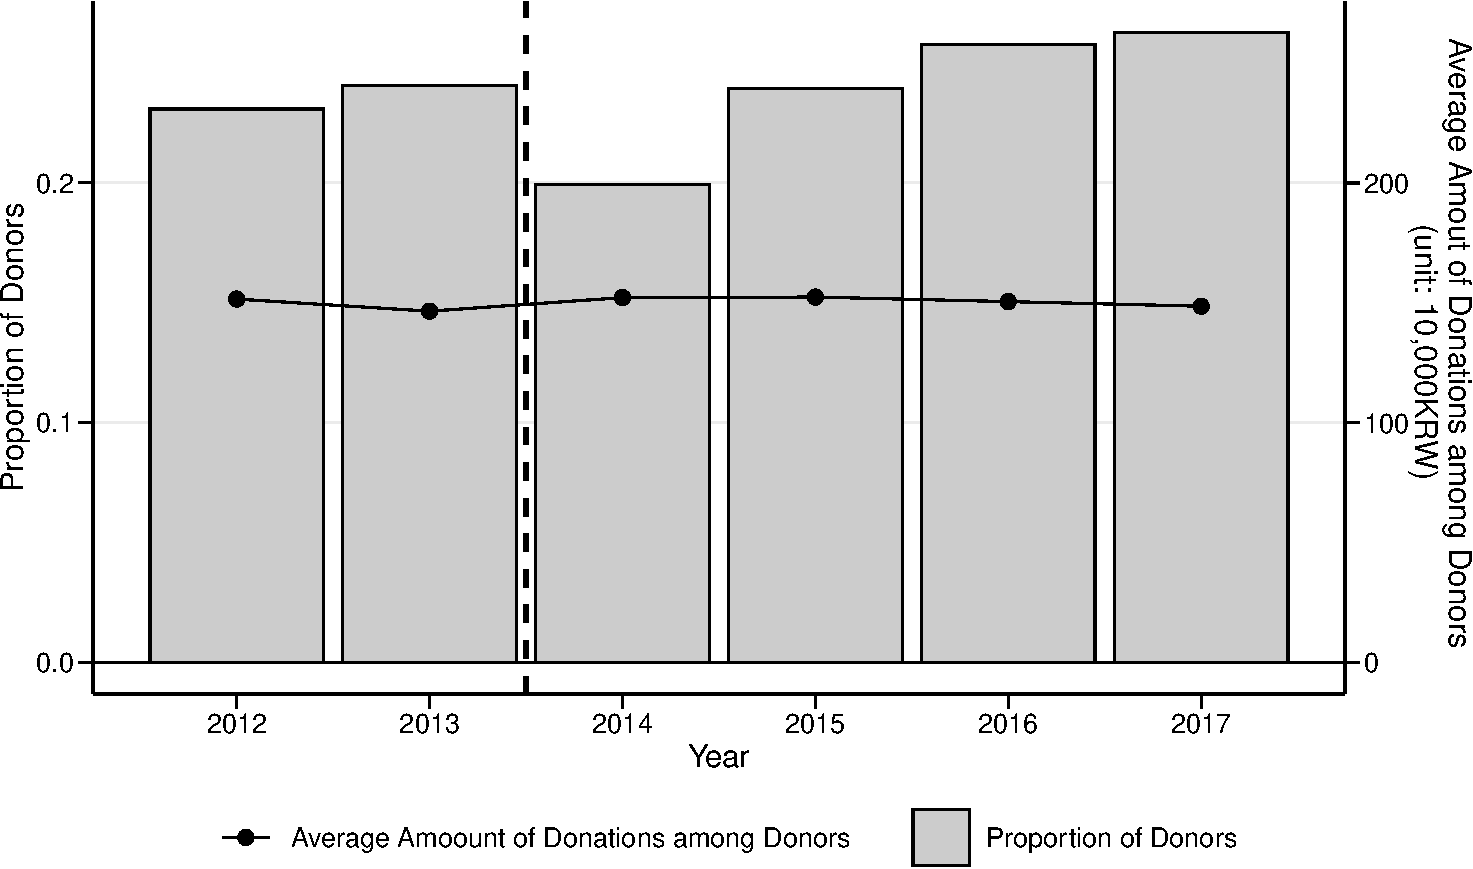
\includegraphics{C:/Users/vge00/Desktop/NaSTaB/docs/paper/body_files/figure-latex/SummaryGiving-1} 

}

\caption{Proportion of Donors and Average Donations among Donors. Notes: The left and right axises measure prooortion of donors (grey bars) and the average amount of donations among donors (solid line), respectively.}\label{fig:SummaryGiving}
\end{figure}

各所得グループの寄付のトレンドを確認する前に、
全体的な寄付行動の傾向を図\ref{fig:SummaryGiving}に示した。
2012年から2017年にかけて、寄付者の割合は約24\%である。
税制改革直後の寄付者の割合は所得控除のもとでの寄付者の割合を下回ったが、
時間を通じて寄付者が増えている(グレーのバー)。
また、寄付者に限定した平均寄付額(黒の実線)は約1.5 million KRW(平均所得の約7\%)
で時間を通じて安定している。
寄付していない人も含めると、平均寄付額は358,600 KRW(平均所得の約2\%)である。

\begin{figure}[t]

{\centering 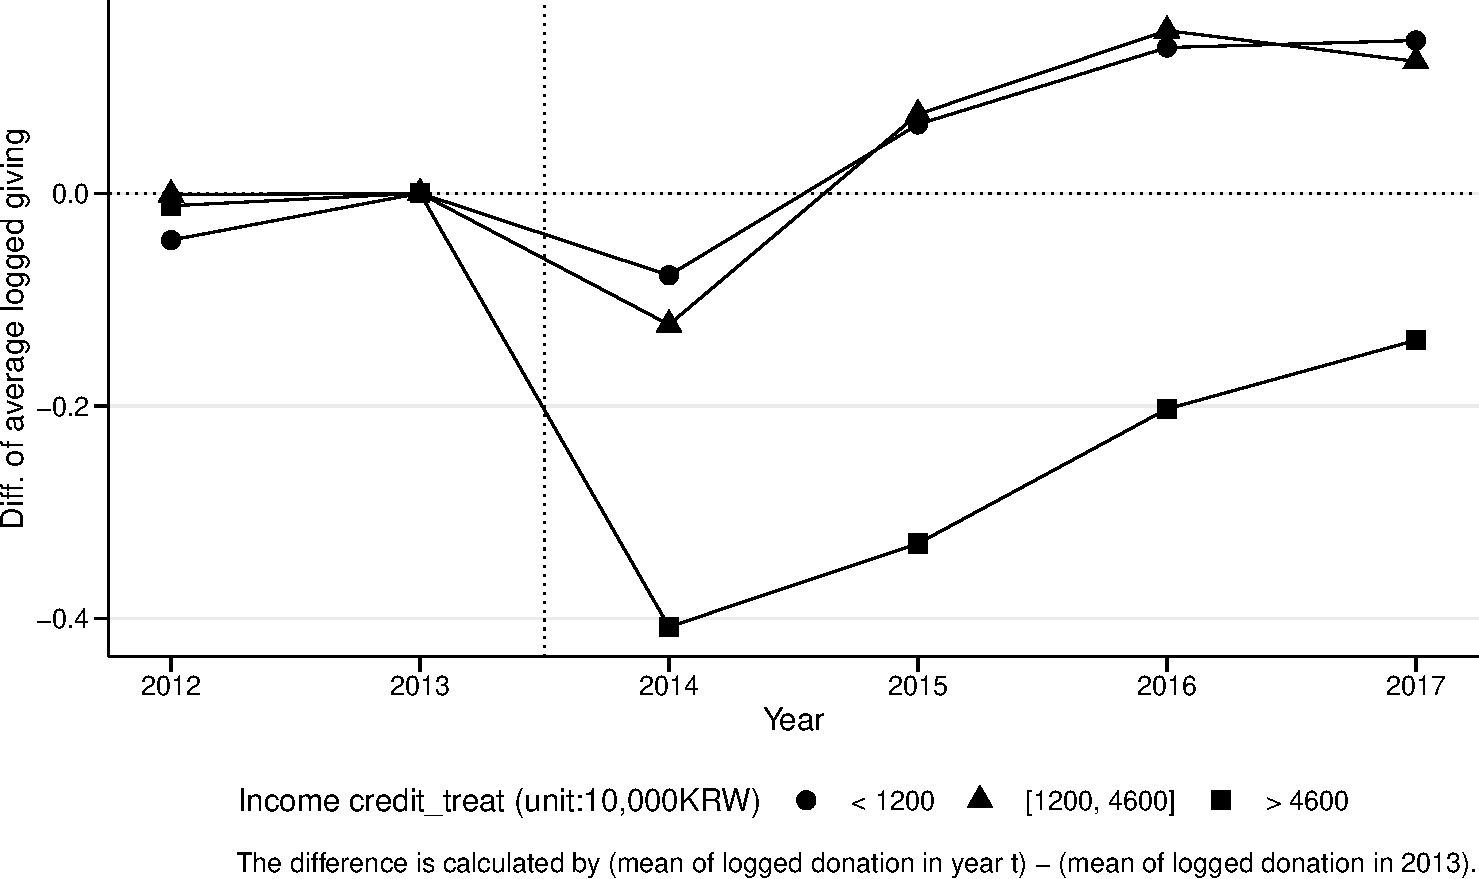
\includegraphics{C:/Users/vge00/Desktop/NaSTaB/docs/paper/body_files/figure-latex/SummaryGivingOverall-1} 

}

\caption{Average Logged Giving by Three Income Groups. Notes: We created three income groups, with the relative price of giving rising (circle), unchanged (triangle), and falling (square) between 2013 and 2014. The group averages are normalized to be zero in 2013.}\label{fig:SummaryGivingOverall}
\end{figure}

図\ref{fig:SummaryGivingOverall}は
税インセンティブの変化に基づいた所得グループごとの平均寄付額を示している(非寄付者も含めている)。
この図から価格効果を観察できる。言い換えれば、税インセンティブは寄付行動を促進していることが観察される。
2015年以降、税制改革によって税インセンティブが拡大した(もしくは変化しなかった)人は所得控除時よりも増えているが、
税インセンティブが縮小した人は所得控除時よりも減少している。
また、寄付者に限定した平均寄付額と寄付者の割合のトレンドを所得グループごとに見ると、
似たような傾向が観察された
(補論を参照せよ)。
ただし、寄付者に限定した平均寄付のトレンドを見ると、
図\ref{fig:SummaryGivingOverall}ほどはっきりとした価格効果を観察できない。

また、すべての所得グループの2014年の平均寄付額は2013年のそれを下回っている。
これはいくつかの可能性が考えられる。
第一に、税制改革のアナウンスメント効果である。
2014年の税制改革は2013年に告知されているので、
税インセンティブが縮小する所得グループにおいては、
2013年の寄付額を増やし、2014年の寄付額を減らすという異時点間の代替効果が予想される。
しかしながら、これは税インセンティブが拡大する所得グループの寄付額が減少した事実を説明できない。
第二の可能性は、制度の学習効果が考えられる。
税制改革直後は、税額控除によって自分が寄付によって節税しやすくなったかどうかが分からないので、
税インセンティブが拡大する所得グループでも寄付額は減少した。
それ以降、税インセンティブが拡大した納税者は自分が寄付によって節税しやすくなることを学習し、
寄付額を所得控除時よりも増やしたと考えられる。

寄付価格の変動は寄付控除の申告の有無でも生じる。
寄付控除を申告した場合の寄付の相対価格は図\ref{fig:SummaryPrice}に示した通りである一方で、
寄付控除を申告しない場合の寄付の相対価格は1である。
よって、控除の有無によって寄付の相対価格は変化する。
しかしながら、寄付控除の申告は自己選択なので、内生的である。
後に述べるように、この内生性を解決するために操作変数が必要である。

寄付控除の申告行動において、申告コストは大きな障害となっている可能性が高い。
補論\ref{addtab}の図\ref{fig:SummaryGivingIntensiveDist}に示しているように、
寄付控除の申告の有無によって、寄付者に限定した寄付額の分布は大きく変化しない。
これは寄付控除の申告の有無は、控除によって得られる便益の差よりも
申告するためのコストの差で説明できることを示唆している。

\begin{figure}[t]

{\centering 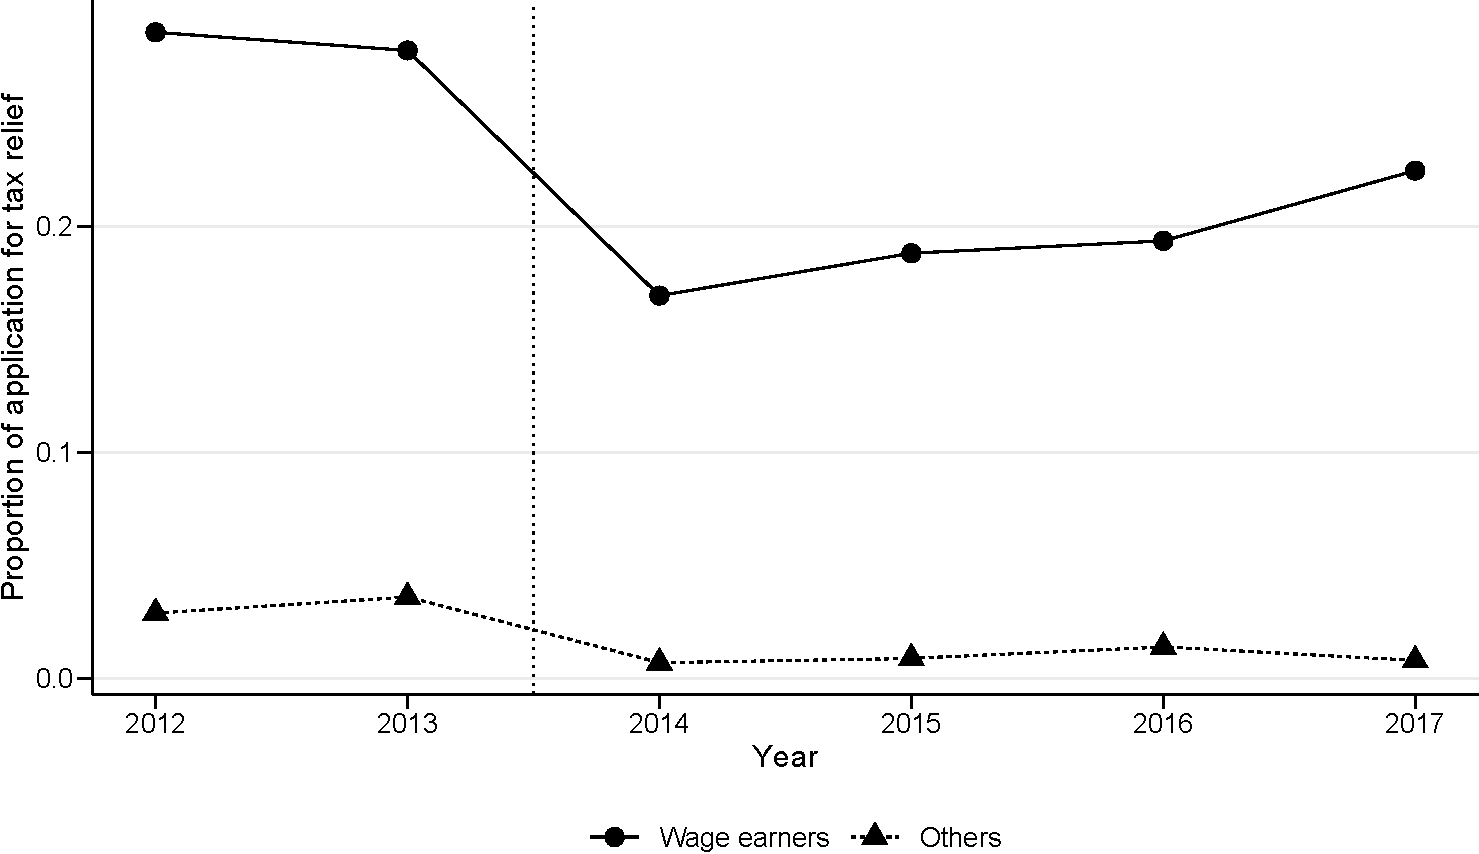
\includegraphics{C:/Users/vge00/Desktop/NaSTaB/docs/paper/body_files/figure-latex/SummaryReliefbyEarner-1} 

}

\caption{Share of Tax Relief by Wage Earners. Notes: A solid line is the share of applying for tax relief among wage eaners. A dashed line is the share of applying for tax relief other than wage earners.}\label{fig:SummaryReliefbyEarner}
\end{figure}

以上を踏まえて、
我々は申告コストの要素の一つであるレコードキーピングに関する制度背景を第二の識別戦略として用いる。
先に述べたように、自営業者は寄付控除を申請するまで寄付の領収書(証明書)を保持しておく必要がある一方で、
給与所得者は会社を通じてその証明書をいつでも提出でき、
その後の申請も会社に手続きを依頼できる。
すなわち、給与所得者は自営業者よりも申告コストが低いことが予想される。
事実、図\ref{fig:SummaryReliefbyEarner}
給与所得者の控除の申請比率は自営業者よりもすべての期間を通じて高いことが分かる\footnote{寄付者に限定した控除の申告比率についても、給与所得者の方が自営業者よりも高い
  (補論\ref{addtab}の図\ref{fig:SummaryReliefbyEarner2})。}。
我々は給与所得者ダミーをレコードキーピングのコストの代理変数として操作変数に用いる。

\hypertarget{estimation}{%
\section{Empirical Strategy}\label{estimation}}

Almunia et al. (2020) に従い、我々は二種類の弾力性を推定する。
第一に、intensive-margin price elasiticityであり、
1\%の価格上昇で寄付者の寄付額が何\%増えるかを示している。
第二に、extensive-margin price elasiticityであり、
1\%の価格上昇で寄付者比率が何\%増えるかを示している。
第\ref{nastab}節で説明したように、
我々は2014年の税制改革による税インセンティブの変化を用いたDIDと
申告コストによる寄付控除の申請の有無を捉えた操作変数法の二つを組み合わせた識別戦略を用いる。

intensive-margin price elasticityは、
寄付者に限定して以下のtwo-way fixed effect modelを推定する。
\begin{align}
  \ln g_{it} = \theta_i + \gamma (R_{it} \times \ln (1 - s_{it}))
    + \beta X_{it} + \lambda_t + u_{it}, \label{eq:intensive}
\end{align}
ここで、\(X_{it}\)は課税前所得(\(y_{it}\))を含んだ共変量ベクトル、
\(\theta_i\)と\(\lambda_t\)はそれぞれ個人固定効果と時間固定効果である。
\(u_{it}\)はidiosyncratic errorである。
アウトカム変数\(\ln g_{it}\)は\(t\)年に寄付した人\(i\)の寄付額の対数値である。
寄付価格は\(R_{it} \times \ln (1 - s_{it})\)であり、
ここで、\(R_{it}\)は控除申請のダミー変数、\(s_{it}\)は税インセンティブである\footnote{寄付価格は\(\ln(1 - R_{it}s_{it})\)とも書ける。
  これは\(R_{it} \times \ln (1 - s_{it})\)と一致する。
  なぜなら、\(R_{it} = 0\)のとき、\(\ln(1) = 0\)となり、
  \(R_{it} = 1\)のとき、\(\ln(1 - s_{it})\)となる。}。
したがって、関心のあるパラメータは\(\gamma\)であり、
これがintensive-margin price elasticityを示す。

extensive-margin price elasticityの推定式は
two-way fixed effect付きの線形確率モデルである。
すなわち、
\begin{align}
  D_{it} = \theta_i + \delta (R_{it} \times \ln (1 - s_{it}))
    + \beta X_{it} + \lambda_t + \eta_{it}, \label{eq:extensive}
\end{align}
である。
アウトカム変数\(D_{it}\)は正の寄付額が観測されたら1を取るダミー変数である:\(D_{it} = 1[g_{it} > 0]\)。
ここで関心のあるパラメータは\(\delta\)である。
アウトカム変数は二値なので、このパラメータを弾力性として直接解釈できない。
extensive-margin price elasticityは\(\hat{\delta} / \bar{D}\)で得られる
(\(\bar{D}\)は\(D_{it}\)の標本平均)。

この推定式における二つの内生性に対する対処法について議論する。
第一に、
2014年の税制改革による税インセンティブの変化を寄付価格の外生的な変動要因として用いるが、
寄付価格の内生性は完全に排除できない。
寄付控除を申請した場合の寄付価格を以下のようになる。
\begin{align}
  1 - s_{it} =
  \begin{cases}
    1 - T'_t(y_{it} - g_{it})  \quad\text{if}\quad t < 2014  \\
    1 - m \quad\text{if}\quad t \ge 2014
  \end{cases},
\end{align}
ここで、\(T'_t(\cdot)\)は\(t\)年の限界所得税率、\(m\)は税額控除率(\(m = 0.15\))である。
寄付価格は2014年の税制改革だけではなく、
所得控除が適用される期間において、寄付額(\(g_{it}\))にも依存する。
これは\emph{last}-unit priceと呼ばれるものであり、この寄付価格は寄付額について内生的である\footnote{寄付額によるインセンティブの操作について、次の二つの可能性が考えられる。
  第一に、納税者は寄付額を減らすことで、所得税率を高められる(寄付価格を高められる)。
  第二に、納税者は寄付額を増やすことで、所得税率を下げられる(節税の額を増やせる)。}。

本研究は、過去の研究にならい、
last-unit priceの代わり(もしくはその操作変数)として\emph{first}-unit priceを用いる。
last-unit priceは最終的な寄付額で寄付価格を計算する一方で、
first-unit priceは寄付額をゼロとして寄付価格を計算する\footnote{first-unit priceは
  最初の1単位を寄付するかどうかの意思決定時に直面する価格として解釈できる。}。
すなわち、
\begin{align}
  1 - s^f_{it} =
  \begin{cases}
    1 - T'_t(y_{it} - 0)  \quad\text{if}\quad t < 2014  \\
    1 - m \quad\text{if}\quad t \ge 2014
  \end{cases}.
\end{align}
ただし、税額控除が適用される期間においては、
寄付価格が寄付額に依存しないので、last-unit priceとfirst-unit priceは一致する。

第二に、寄付控除申告の自己選択による内生性である。
申告コストがないとき、節税による便益を得られるので、
寄付者は全員寄付控除を申請するべきである。
しかしながら、我々のデータでは、寄付者の割合は24\%であるにも関わらず、
控除を申告した人の割合は10\%である(表\ref{tab:SummaryCovariate})。
また、補論\ref{addtab}の図\ref{fig:SummaryGivingIntensiveDist}に示しているように、
寄付控除の申告の有無によって、寄付者に限定した寄付額の分布は大きく変化しない。
これは寄付控除の申告行動において、申告コストは大きな障害となっている可能性が高いことを示唆している。

本研究はレコードキーピングの制度が給与所得者と自営業者で異なることを利用して、
給与所得者ダミー(\(WE_{it}\))をレコードキーピングのコストの代理変数として操作変数に用いる\footnote{給与所得者ダミーを操作変数として用いるためには、
  共変量で条件づけたとき、この変数が\(u_{it}\)と\(\eta_{it}\)と独立していることを仮定する必要がある。
  ただし、給与所得者ダミーと固定効果の相関は許容できる。
  我々は、所得や業種をコントロールすれば、
  給与所得者であるかどうかは寄付行動に直接的な影響を持たないと考えている。}。
自営業者は寄付控除を申請するまで寄付の領収書(証明書)を保持しておく必要がある一方で、
給与所得者は会社を通じてその証明書をいつでも提出できるので、
給与所得者は自営業者よりも申告コストが低いことが予想される。

Wooldridge (2010) に従い、
我々は給与所得者ダミーを操作変数とした三つのアプローチを用いる\footnote{以降ではintensive-margin price elasticityの推定式を用いて説明するが、
  extensive-margin price elasticityの推定についても同じ方法が適用できる。}。
第一に、給与所得者ダミーとfirst-unit priceの交差項を
\(R_{it} \times \ln (1 - s^f_{it})\)の操作変数として用いる。
すなわち、intensive-margin price elasiticityの推定式は
\begin{align}
  \ln g_{it} = \theta_i + \gamma (R_{it} \times \ln (1 - s^f_{it}))
    + \beta X_{it} + \lambda_t + u_{it}, \label{eq:intensive2}
\end{align}
であり、
\(R_{it} \times \ln (1 - s^f_{it})\)の操作変数を\(WE_{it} \times \ln(1 - s^f_{it})\)とする\footnote{last-unit priceを用いて弾力性を推定する場合、
  \eqref{eq:intensive}もしくは\eqref{eq:extensive}の説明変数
  \(R_{it} \times \ln (1 - s_{it})\)の操作変数として
  \(WE_{it} \times \ln(1 - s^f_{it})\)を用いる。}。

残りの二つのアプローチは寄付申告の傾向スコアを用いるものである。
傾向スコアは以下のモデルをプロビット推定した予測確率で得られる。
\begin{align}
  R_{it} = 1[
    \alpha_0 + \alpha_1 WE_{it} + \alpha_2 \ln(1 - s^f_{it})
    + \alpha_3 X_{it} + u_{it0} > 0
  ] \label{eq:selection}
\end{align}

我々は全期間のサンプルを用いた推定(pooled model)と
年で分割したサブサンプルを用いた推定(separeted model)で傾向スコア\(\hat{P}_{it}\)を得た。
前者のモデルは式\eqref{eq:selection}の係数が時間に対して一定であると仮定している一方で、
後者のモデルは推定される係数が時間に依存することを許容したモデルである。

傾向スコアを用いた第二のアプローチは
式\eqref{eq:intensive2}の説明変数\(R_{it} \times \ln (1 - s^f_{it})\)の操作変数として
\(\hat{P}_{it} \times \ln (1 - s^f_{it})\)を用いる。
第三のアプローチは式\eqref{eq:intensive2}の説明変数\(R_{it} \times \ln (1 - s^f_{it})\)
の代わりに\(\hat{P}_{it} \times \ln (1 - s^f_{it})\)を用いる。すなわち、
我々は以下のモデルを推定する。
\begin{align}
  \ln g_{it} = \theta_i + \gamma (\hat{P}_{it} \times \ln (1 - s^f_{it}))
    + \beta X_{it} + \lambda_t + u_{it}, \label{eq:intensive3}
\end{align}

\hypertarget{result}{%
\section{Estimation Results}\label{result}}

\hypertarget{references}{%
\section*{References}\label{references}}
\addcontentsline{toc}{section}{References}

\hypertarget{refs}{}
\begin{CSLReferences}{1}{0}
\leavevmode\vadjust pre{\hypertarget{ref-Scharf2020}{}}%
Almunia, M., Guceri, I., Lockwood, B., Scharf, K., 2020. More giving or more givers? {The} effects of tax incentives on charitable donations in the {UK}. Journal of Public Economics 183, 104114. doi:\href{https://doi.org/10.1016/j.jpubeco.2019.104114}{10.1016/j.jpubeco.2019.104114}

\leavevmode\vadjust pre{\hypertarget{ref-Wooldridge2010}{}}%
Wooldridge, J.M., 2010. Econometric analysis of cross section and panel data, 2nd ed. ed. {MIT Press}, {Cambridge, Mass}.

\end{CSLReferences}

\end{document}
